% AQC 논문 한국어 번역본
% 원문: ../../AQC/main.tex
\documentclass[twocolumn,a4paper]{article}

\usepackage{../../AQC/nolta2025}
\usepackage{kotex}
\usepackage{amsmath,amssymb,bbm,graphicx,subcaption,color,physics,hyperref,algorithm,algorithmic,txfonts}

\DeclareMathOperator*{\argmax}{arg\,max}
\DeclareMathOperator*{\argmin}{arg\,min}

\newcommand{\inp}[2]{\left\langle {#1} \middle| {#2} \right\rangle}
\newcommand{\kb}[1]{\ket{{#1}}\!\bra{{#1}}}
\newcommand{\bbE}{\mathbb{E}} \newcommand{\bbN}{\mathbb{N}} \newcommand{\bbB}{\mathbb{B}}
\newcommand{\bbS}{\mathbb{S}} \newcommand{\bbR}{\mathbb{R}} \newcommand{\bbC}{\mathbb{C}}
\newcommand{\bbZ}{\mathbb{Z}} \newcommand{\bbH}{\mathbb{H}} \newcommand{\bbQ}{\mathbb{Q}}
\newcommand{\calX}{\mathcal{X}} \newcommand{\calY}{\mathcal{Y}} \newcommand{\calZ}{\mathcal{Z}}
\newcommand{\calH}{\mathcal{H}} \newcommand{\calV}{\mathcal{V}} \newcommand{\BSC}{\mathrm{BSC}}

\newtheorem{theorem}{정리}
\newtheorem{corollary}[theorem]{따름정리}
\newtheorem{lemma}[theorem]{보조정리}
\newtheorem{proposition}[theorem]{명제}
\newtheorem{remark}{비고}
\newtheorem{example}{예}
\newtheorem{definition}{정의}
\newtheorem{conjecture}{추측}
\newtheorem{postulate}{공준}
\newtheorem{question}{질문}
\newtheorem{observation}{관찰}

\newenvironment{proof}{\par\noindent\textit{증명.}\ }{\hfill\(\square\)\par\medskip}

\begin{document}

\title{군중 압사 사고 예방을 위한 양자 어닐링 기반 보행자 네트워크 방향 최적화: QUBO 정식화 연구}
\author{이요환${}^\dag$, 정윤성${}^\dag$, 김세엽${}^\dag$, 황원주${}^\ddag$}
\address{\dag 부산대학교 정보컴퓨터공학부 \\
\ddag 부산대학교 정보융합공학과 \\
대한민국 부산광역시 46241 \\
Email: \email{dev.vackam@gmail.com}, \email{me@yunseong.dev}, \email{ksy1001k96@gmail.com}, \email{wjhwang@pusan.ac.kr}}
\maketitle

\abstract
좁은 도시 공간에서 서로 반대 방향으로 이동하는 고밀도 보행 흐름이 합류하면 개인의 이동성과 통제력이 심각하게 상실되어 군중 압사 사고가 발생할 수 있다. 본 연구는 이 문제를 해결하기 위해 양자 어닐링 기반 보행자 네트워크 방향 최적화 프레임워크를 제안한다. 보행자 네트워크는 교차점을 정점으로, 보행 가능한 경로를 간선으로 나타내는 가중 그래프로 모델링한다. 최적화 목적은 경로에 통행 방향을 할당하여 보행 흐름 간 충돌을 줄이고, 이동 효율을 높이며, 국부 혼잡을 완화하는 것이다. 이를 위해 세 가지 상호 보완 전략을 통합한다. 사이클 기반 접근법은 전역 순환과 네트워크 연결성을 보존하고, $n$-홉 기반 접근법은 전체 이동 거리를 줄이며, 흐름 보존 접근법은 각 노드의 유입량과 유출량을 균형 있게 만든다. 최종 최적화 문제는 이차 비제약 이진 최적화(Quadratic Unconstrained Binary Optimization, QUBO) 모델로 정식화하고 D-Wave 양자 어닐링 플랫폼에서 푼다. 실험 결과, 제안 방법은 기존 접근법보다 적은 계산 시간을 요구하면서 혼잡을 줄이고 흐름 안정성을 개선하며 모든 쌍 최단 경로(APSP)의 합을 낮추는 것으로 나타났다.
\endabstract

\section{서론} \label{sec:intro}

군중 압사 사고는 중대한 공공 안전 문제이며 여러 상황에서 심각한 인명 피해를 일으켰다~\cite{fruin1993causes}. 이러한 사고는 단순히 높은 인구 밀도 때문에 발생하는 것이 아니라 지형적 제약과 병목 같은 환경 조건~\cite{helbing2007dynamics}, 쓰러진 사람에 대한 불충분한 초기 대응~\cite{soomaroo2012disasters} 등 여러 요인의 복잡한 상호작용에서 비롯된다. 2022년 대한민국에서 발생한 군중 사고는 제한된 도시 공간의 극심한 혼잡이 얼마나 빠르게 치명적 상황으로 이어질 수 있는지를 보여 준다~\cite{chang2024crowd}.

이러한 군중 관련 사고를 예방하기 위해 다양한 다면적 해결책이 연구되어 왔다~\cite{Nishinari2024}. 그러나 실제 도시 환경은 매우 광대하고 복잡하며 도로 폐쇄와 병목 같은 예측하지 못한 변수가 동시에 실시간으로 발생한다. 동적으로 변화하는 대규모 환경에서 모든 변수를 고려하고 실시간 최적해를 도출하기 위해 고전 컴퓨팅 자원에만 의존하는 데에는 명확한 한계가 있다.

본 연구는 이러한 문제를 극복하기 위해 대상 지역의 공간적 특성을 그래프로 추상화한다. 양자 어닐링의 기초 프레임워크~\cite{Kadowaki1998}를 바탕으로 군중 제어 최적화 문제를 QUBO 모델로 직접 정식화한다. 이 정식화를 통해 양자 하드웨어를 효과적으로 활용하여 최적 경로를 빠르게 도출하고, 대규모 혼잡 상황에서 군중 밀도를 최소화할 수 있다.

본 연구의 기여는 다음과 같다.
\begin{itemize}
    \setlength{\itemsep}{0pt}
    \setlength{\parsep}{0pt}
    \setlength{\parskip}{0pt}
    \item[(1)] 복잡한 도시 네트워크와 동적 흐름을 포착하는 그래프로 군중 제어 문제를 모델링한다.
    \item[(2)] 양자 어닐링으로 대규모 경로 설정 문제를 효율적으로 풀기 위한 새로운 QUBO 정식화를 제안한다.
    \item[(3)] 고전 알고리즘과의 비교를 통해 실시간 재난 대응에 양자 컴퓨팅을 적용할 수 있음을 보인다.
\end{itemize}

이후 구성은 다음과 같다. 제~\ref{sec:related}절에서 관련 연구를 검토하고, 제~\ref{sec:method}절에서 제안 방법을 설명한다. 제~\ref{sec:result}절에서 시뮬레이션 결과를 제시하고, 마지막으로 제~\ref{sec:conclusion}절에서 결론을 맺는다.

\section{관련 연구} \label{sec:related}

\subsection{군중 안전과 보행 흐름 제어} \label{subsec:related_crowd}

군중 안전에 관한 선행 연구는 미시적 군중 시뮬레이션, 대피 모델, 흐름 기반 접근법으로 보행자 이동을 분석해 왔다. 이들 연구는 보행자 사이의 밀집 상호작용이 보행 속도를 낮추고 국부 병목을 만들며 불안정한 군중 이동의 위험을 높일 수 있음을 보였다. 교통 및 대피 계획 분야에서는 비상 상황에서 일부 통행 방향을 역전하여 도로 용량 활용도를 높이는 역류(contraflow) 전략도 연구되었다~\cite{kim2008contraflow, aksu2014mathematical}.

그러나 기존 접근법 다수는 보행자 순환 네트워크의 구조 설계보다 운영상 군중 관리나 시뮬레이션 기반 분석에 초점을 둔다. 특히 예방적 인프라 대책으로서 일방통행 보행 경로의 방향을 최적화하는 연구는 상대적으로 부족하다.

\subsection{그래프 기반 네트워크 방향 설정} \label{subsec:related_graph}

무방향 그래프의 간선에 방향을 할당하는 문제는 그래프 이론에서 폭넓게 연구되었다. 고전 연구는 강한 연결성을 유지하면서 무방향 그래프에 방향을 부여할 수 있는 조건을 확립했다~\cite{robbins1939theorem}. 후속 연구에서는 강연결 방향 설정, 네트워크 신뢰성, 교통 네트워크의 최적 방향 할당을 다루었다~\cite{chung1985strongly, roberts1988optimal, roberts1994optimal}.

일방통행 도로 설계 또한 교통 네트워크 최적화 문제로 연구되었다. 기존 접근법은 일반적으로 이동 시간 단축, 교통 용량 개선 또는 도로망 변경 비용 최소화를 목표로 한다~\cite{drezner1997selecting, huang2020bi, huang2020model}. 그러나 간선 수에 따라 가능한 방향 할당 수가 지수적으로 증가하므로 네트워크가 커질수록 계산이 어려워진다. 강한 연결성, 아크 역전, 여러 최적화 목적을 동시에 고려하면 복잡도는 더욱 커진다~\cite{burkard1999minimum, bangjensen2023complexity}.

차량 교통에 주로 초점을 맞춘 선행 연구와 달리 본 연구는 보행자 안전 중심의 네트워크 방향 설정을 다룬다. 제안 정식화는 국부 흐름 균형, 짧은 경로 도달 가능성, 순환 보존을 명시적으로 결합한다.

\subsection{조합 최적화를 위한 양자 어닐링} \label{subsec:related_qa}

양자 어닐링은 Ising 또는 QUBO 형태로 표현할 수 있는 여러 조합 최적화 문제에 적용되어 왔다~\cite{qa_for_optimize}. 대표 응용 분야로 경로 설정, 스케줄링, 그래프 분할, 자원 할당이 있다. QUBO 모델은 이진 결정 변수와 변수 간 쌍별 상호작용을 에너지 함수에 부호화하여 양자 어닐러가 낮은 에너지의 후보 해를 탐색할 수 있게 한다.

현재 양자 어닐링 하드웨어에서 실제로 실행하려면 논리 변수와 그 상호작용을 연결성이 제한된 물리 큐비트에 매핑하는 마이너 임베딩이 필요하다~\cite{minor_embedding_inQA2, minor_embedding_inQA}. 이 과정에서는 하나의 논리 변수가 여러 물리 큐비트로 이루어진 체인을 요구할 수 있어 추가 오버헤드가 발생한다. 따라서 QA 호환 최적화 모델을 설계할 때 임베딩의 실현 가능성과 품질을 고려해야 한다.

이러한 연구를 바탕으로 본 연구는 보행자 네트워크 방향 설정 문제를 QUBO 모델로 정식화하고 D-Wave 양자 어닐링 플랫폼에서 적용 가능성을 평가한다.

\section{시스템 모델과 문제 정식화} \label{sec:model}

\subsection{보행자 네트워크와 결정 변수} \label{subsec:model_graph}

가중 무방향 그래프 $G=(V,E,W)$로 표현되는 도시 보행 환경을 고려한다. 여기서 \(V\)는 보행자 교차점, 분기점 또는 의사결정 지점의 집합이고, \(E\)는 이들을 연결하는 보행 가능 구간의 집합이다. 각 무방향 간선 \(\{i,j\}\in E\)는 원래 양방향 이동이 가능한 물리적 보행로를 나타낸다. 다리(bridge)를 포함하는 그래프는 강연결 방향 설정 자체가 불가능하므로~\cite{robbins1939theorem}, 본 연구는 평면 근사와 무다리 가정이 성립하는 지상 보행망으로 대상을 한정하여 \(G\)가 평면이고 연결되어 있으며 다리를 갖지 않는다고 가정한다. 이때 모든 블록이 이중연결이 되어 면 구조가 잘 정의된다. 실험에서는 Delaunay 삼각분할로 생성한 평면 그래프를 사용한다.

각 간선의 가중치 \(w_{ij}\geq1\)은 단위 폭을 기준으로 한 유효 폭과 보행 용량을 나타낸다. 따라서 해당 구간의 통과 비용, 즉 거리는 그 역수
\begin{equation}
    \ell_{ij}=\frac{1}{w_{ij}}
\end{equation}
로 정의한다. 넓고 용량이 큰 경로일수록 통과 비용이 작다. 고밀도 보행 환경에서 좁은 경로의 양방향 이동은 대향 흐름 충돌을 일으키고 보행 효율을 낮추며 국부 혼잡 위험을 높일 수 있다. 따라서 본 연구의 목적은 각 보행 구간에 하나의 보행 방향을 할당하여 기존 양방향 보행자 네트워크를 방향성 일방통행 순환 네트워크로 변환하는 것이다.

각 무방향 간선 \(\{i,j\}\in E\)에 대해 끝점이 \(i<j\)를 만족하도록 임의의 고정 순서를 두고, 이진 방향 변수 \(x_{ij}\)를 \(x_{ij}=0\)이면 \(i\rightarrow j\), \(x_{ij}=1\)이면 \(j\rightarrow i\)로 정의한다. 전체 변수 벡터 \(\mathbf{X}\in\{0,1\}^{|E|}\)는 방향 그래프 \(\vec{G}(\mathbf{X})=(V,\vec{E}(\mathbf{X}))\)를 완전히 결정하며, 각 물리적 보행 구간에는 정확히 하나의 방향이 할당된다. 이하의 정의는 표기를 간결히 하기 위해 끝점 쌍으로 첨자를 쓰지만, 축약을 거치면 같은 끝점 쌍을 잇는 간선이 둘 이상 생길 수 있다. 그 경우 변수와 지시 함수는 간선 식별자로 구분하고, \(\mathrm{adj}(v)\)에 대한 합은 모두 \(v\)에 입사하는 간선에 대한 합으로 읽는다. 이 구성은 원래 네트워크의 공간 위상을 보존하면서 개별 보행로의 대향 흐름을 제거한다.

이후 서술을 간결하게 하기 위해 인접한 노드의 순서쌍 \((a,b)\)에 대한 방향 지시 함수를 먼저 정의한다.
\(\{a,b\}\in E\)일 때 \(a<b\)이면 \(\rho_{ab}(\mathbf{X})=1-x_{ab}\), \(b<a\)이면 \(\rho_{ab}(\mathbf{X})=x_{ba}\)로 둔다.
\(\rho_{ab}\)는 추가 결정 변수가 아니라 \(\mathbf{X}\)로 완전히 결정되는 표현이며, \(\vec{G}(\mathbf{X})\)에 \(a\rightarrow b\)가 있으면 1이고 항상 \(\rho_{ab}+\rho_{ba}=1\)이다. \(v\)에 인접한 정점 집합은 \(\mathrm{adj}(v)\)로 둔다.

\subsection{흐름 보존 목적함수} \label{subsec:model_flow}

교차점에서 유입 흐름과 유출 흐름의 차이가 크면 바람직하지 않은 순환 패턴이 생길 수 있다. 유입은 많고 유출은 적은 노드는 구조적 누적 지점이 되어 군중이 쌓이고, 반대인 노드는 인근 지역의 접근성을 떨어뜨린다. 보행 구간의 수용 능력이 서로 다르므로 불균형은 방향의 개수가 아니라 용량으로 측정한다. 노드 \(v\)의 유출 용량과 유입 용량을 각각
\begin{equation}
d_v^{+}(\mathbf{X})=\!\!\sum_{u\in\mathrm{adj}(v)}\!\!w_{vu}\rho_{vu},
\qquad
d_v^{-}(\mathbf{X})=\!\!\sum_{u\in\mathrm{adj}(v)}\!\!w_{vu}\rho_{uv}
\end{equation}
로 두면 \(\rho_{vu}+\rho_{uv}=1\)에서 \(d_v^{+}+d_v^{-}=\sum_{u}w_{vu}\)가 성립한다. 노드 \(v\)의 방향 불균형은
\begin{equation}
B_v(\mathbf{X})=d_v^{+}(\mathbf{X})-d_v^{-}(\mathbf{X})=\!\!\sum_{u\in\mathrm{adj}(v)}\!\!w_{vu}\left(2\rho_{vu}-1\right)
\end{equation}
이며, 국부 흐름 균형 목적함수는
\begin{equation}
F_{\mathrm{bal}}(\mathbf{X})=\sum_{v\in V}B_v(\mathbf{X})^2
\label{eq:fflow}
\end{equation}
이다. 이를 최소화하면 각 노드의 유입 용량과 유출 용량이 비슷해진다. 단위 가중치에서는 \(B_v\equiv\deg(v)\ (\mathrm{mod}\ 2)\)이므로 \(B_v^2\)의 하한이 정점마다 차수 패리티로 정해지고, 홀수 차수 정점을 짝지어 보조 간선으로 이은 뒤 오일러 회로를 따라 배향하면 모든 정점이 그 하한에 동시에 도달하므로 \(F_{\mathrm{bal}}\) 단독 최소화가 다항 시간에 풀린다. 그러나 용량 가중치를 쓰면 약한 의미에서 이미 NP-난해하다. PARTITION~\cite{garey1979computers} 사례 \(\{w_i\}\)에 대해 정점 두 개를 길이 2의 내부 서로소 경로 \(n\)개로 잇고 경로 \(i\)의 두 간선에 \(w_i\)를 주면, 경로가 반대로 배향될 때 중간 정점이 \(4w_i^2>0\)을 기여하므로 목적값 0인 배향에서는 각 경로의 두 간선이 같은 방향이어야 하고 목적값이 \(2(\sum_i\varepsilon_iw_i)^2\)이 된다. 최소값이 0인지 판정하는 것이 곧 PARTITION 판정이며, 이 그래프는 평면이고 다리가 없다.

\subsection{이동 효율 목적함수}

방향성 보행자 네트워크는 국부 균형뿐 아니라 도시 공간의 서로 다른 부분 사이에서 효율적인 이동도 지원해야 한다. \(D_{st}(\mathbf{X})\)를 \(\vec{G}(\mathbf{X})\)에서 간선 거리 \(\ell_{ij}=1/w_{ij}\)에 따라 계산한 출발 노드 \(s\)부터 도착 노드 \(t\)까지의 최단 방향 경로 거리라 하고, \(\bar{D}_{st}\)를 방향화 이전 무방향 그래프 \(G\)에서의 대응 최단 거리라 하자. \(s\)에서 \(t\)로 가는 방향 경로가 없으면 \(D_{st}(\mathbf{X})=\infty\)로 둔다.

방향화가 거리를 얼마나 늘리는지는 그래프 이론에서 오래 연구되었다~\cite{chvatal1978distances}. 본 연구는 이동 효율을 절대 거리의 합이 아니라 방향화로 인해 늘어난 우회 비율로 측정한다. 정규화된 모든 쌍 최단 경로 비용을
\begin{equation}
F_{\mathrm{dist}}(\mathbf{X})=\frac{1}{|V|(|V|-1)}\sum_{\substack{s,t\in V\\s\neq t}}\frac{D_{st}(\mathbf{X})}{\bar{D}_{st}}
\label{eq:stretch}
\end{equation}
로 정의한다. 항상 \(D_{st}\geq\bar{D}_{st}\)이므로 \(F_{\mathrm{dist}}(\mathbf{X})\geq1\)이고, 값이 1에 가까울수록 방향화가 원래의 보행 거리를 잘 보존한다. 이 지표는 그래프 크기와 가중치 스케일에 불변이므로 서로 다른 규모의 네트워크를 비교할 수 있다. 다만 제~\ref{sec:result}절의 실험은 정규화하지 않은 평균 유향 거리를 기록하였으므로 크기 간 비교에는 쓸 수 없다.

식~\eqref{eq:stretch}가 의미를 가지려면 \(\vec{G}(\mathbf{X})\)가 강연결이어야 한다. \(\vec{G}(\mathbf{X})\)가 강연결이 되는 \(\mathbf{X}\) 전체의 집합을 \(\mathcal{X}_{\mathrm{sc}}\)로 둔다.

\subsection{짧은 경로 도달 가능성 대리 목적함수} \label{subsec:model_hop}

식~\eqref{eq:stretch}의 \(F_{\mathrm{dist}}\)는 전체 그래프의 전역 방향 패턴에 의존하는 비국소 함수이므로 이차식으로 직접 표현할 수 없다. 따라서 짧은 방향 경로 형성을 유도하는 국부 도달 가능성 대리 목적함수를 도입한다. \(\rho\)를 사용하면 서로 다른 노드로 이루어진 길이 \(n\)의 방향 보행 \((v_0,v_1,\dots,v_n)\) 전체에 대한 가중 개수는
\begin{equation}
P_n(\mathbf{X})=\sum_{(v_0,\dots,v_n)}\;\prod_{r=1}^{n}w_{v_{r-1}v_r}\,\rho_{v_{r-1}v_r}(\mathbf{X})
\label{eq:pn}
\end{equation}
로 나타낼 수 있다. 합의 범위는 \(v_r\neq v_{r'}\ (r\neq r')\)이고 \(\{v_{r-1},v_r\}\in E\ (1\leq r\leq n)\)인 보행 전체이며, 평행 간선이 있으면 항은 간선열로 구분되지만 중복 배제는 여전히 정점 기준이다. 정점 중복을 배제하므로 되돌아오는 보행은 세지 않는다.

\(P_n\)은 형식상 \(n\)차이지만, 보행과 그 반전이 짝을 이루면서 최고차가 상쇄될 수 있다.

\begin{proposition} \label{prop:deg}
\(n\geq1\)이라 하고, 간선 중 일부는 방향이 상수로 고정되어 있어도 좋다(제~\ref{subsec:method_pre}절의 사전 배향된 경계 간선). 이때 \(P_n\)은 \(n\)이 홀수이면 차수 \(n-1\) 이하, 짝수이면 차수 \(n\) 이하의 다항식이다. 특히 \(P_2\)와 \(P_3\)는 모두 차수 2 이하다.
\end{proposition}

\begin{proof}
식~\eqref{eq:pn}의 합은 보행의 반전에 대해 닫혀 있고, 정점이 서로 다르므로 \(v_0\neq v_n\)이어서 반전은 고정점 없는 대합이다. 반전 짝의 가중치 곱은 \(w\)의 대칭성에서 서로 같다. 짝이 지나는 간선이 모두 자유이면 \(\rho_r=\rho_{v_{r-1}v_r}\)로 둘 때 반전 보행의 인자가 \(1-\rho_r\)이므로 짝의 합은 \(\prod_rw_r\bigl[\prod_r\rho_r+\prod_r(1-\rho_r)\bigr]\)이다. 정점이 서로 달라 \(n\)개의 간선이 모두 다르고 각 \(\rho_r\)는 \(x_{e_r}\) 또는 \(1-x_{e_r}\)이므로, \(\rho_r=1-x_{e_r}\)인 \(r\)의 개수를 \(k\)라 하면 \(\prod_rx_{e_r}\)의 계수는 앞 항에서 \((-1)^k\), 뒤 항에서 \((-1)^{n-k}\)이고 합이 \((-1)^k\bigl(1+(-1)^n\bigr)\)이다. 따라서 \(n\)이 홀수이면 소거되고 짝수이면 크기가 두 배가 된다. 짝이 지나는 간선 중 하나라도 사전 배향되어 있으면 그 인자는 상수이고 방향이 어긋나는 쪽 보행은 인자가 0이 되어 사라지므로, 남는 항의 변수가 \(n-1\)개 이하여서 그 짝은 홀짝과 무관하게 이미 \(n-1\)차 이하를 기여한다.
\end{proof}

명제~\ref{prop:deg}의 상한은 홀수 \(n\)에서 \(n-1\), 짝수 \(n\)에서 \(n\)이므로 이차식이 보장되는 홉 길이는 \(n\in\{2,3\}\)뿐이며, 이것이 홉 길이를 이 둘로 한정하는 또 하나의 이유다. \(P_n\)은 방향 설정이 단거리·중거리 도달 가능성을 얼마나 지원하는지 측정하며, 이를 최대화하면 불필요한 우회를 줄이는 구조적 대리 지표가 된다. 이에 따라 짧은 경로 도달 가능성 목적함수를
\begin{equation}
F_{\mathrm{hop}}(\mathbf{X})=-\lambda_2P_2(\mathbf{X})-\lambda_3P_3(\mathbf{X})
\end{equation}
로 정의한다.

두 목적함수는 독립이 아니다. \(G\)가 단순 그래프이면 한 간선의 방향이 하나뿐이라 \(\rho_{uv}\rho_{vu}=0\)이므로 식~\eqref{eq:pn}의 정점 중복 배제는 \(n=2\)에서 아무것도 제외하지 않고, 가운데 정점으로 묶으면 \(P_2=\sum_v d_v^{+}d_v^{-}\)이다. 여기에 \(B_v^2=(d_v^{+}+d_v^{-})^2-4d_v^{+}d_v^{-}\)와 \(S_v=\sum_{u}w_{vu}\)가 배향에 무관한 상수임을 쓰면
\begin{equation}
    F_{\mathrm{bal}}(\mathbf{X})=\sum_{v\in V}S_v^2-4P_2(\mathbf{X})
\label{eq:balhop}
\end{equation}
가 성립한다. 즉 흐름 보존 항과 2-홉 항은 상수를 제외하면 같은 이차형식이며, 세 전략 중 흐름 보존과 2-홉은 서로 다른 층위가 아니라 같은 항의 두 해석이다. 다만 축약으로 평행 간선이 생기면 서로 다른 두 평행 간선이 만드는 \(u\rightarrow v\rightarrow u\) 보행이 \(P_2\)에서는 배제되고 \(\sum_v d_v^{+}d_v^{-}\)에는 남으므로 그만큼 등식이 어긋난다.

\(P_n\)과 거리의 상관은 제~\ref{sec:result}절에서 확인되며, 홉 길이 선택의 영향도 같은 절의 절제 실험으로 다룬다.

\subsection{문제 정식화}

이상을 종합하면 보행자 네트워크 방향 설정 문제는 이진 제약 최적화 문제로 정식화된다. 유일한 결정 변수는 이진 방향 벡터 \(\mathbf{X}\)이며, 정확한 목적함수를 사용하면 문제는
\begin{equation}
\min_{\mathbf{X}\in\mathcal{X}_{\mathrm{sc}}}\quad F_{\mathrm{dist}}(\mathbf{X})+\gamma F_{\mathrm{bal}}(\mathbf{X})
\label{eq:exact}
\end{equation}
로 쓸 수 있다. 여기서 \(\gamma\geq0\)이 이동 효율과 국부 혼잡 완화의 상대적 중요도를 조절한다. 본 연구는 \(\gamma\)를 하나의 수치로 고정하지 않고 두 항을 따로 보고하며, 샘플 선택과 최종 순위는 거리 항 단독으로 매긴다. 식~\eqref{eq:exact}는 \(F_{\mathrm{dist}}\)가 비국소적이고 \(\mathcal{X}_{\mathrm{sc}}\)가 비볼록 조합 제약이므로 양자 어닐러에 직접 올릴 수 없다. \(F_{\mathrm{dist}}\)는 최종 평가와 샘플 선택 단계에서만 계산한다.

\section{제안 방법} \label{sec:method}

\subsection{프레임워크 개요}

제안 프레임워크는 초록에서 제시한 세 전략을 서로 다른 층위에 배치한다. 전처리가 군집 사이를 잇는 순환 골격을 먼저 세우고, 이동 효율과 흐름 보존만 \emph{QUBO 에너지 함수}에 남긴다. 이 골격은 전역 강연결 조건을 각 부분 그래프의 강연결이라는 국소 조건으로 낮춘다(명제~\ref{prop:sc}).
\begin{itemize}
    \setlength{\itemsep}{0pt}
    \setlength{\parsep}{0pt}
    \item[(1)] 사이클 기반 전략 $\rightarrow$ 순환 골격 확보 $\rightarrow$ 전처리(제~\ref{subsec:method_pre}절)
    \item[(2)] $n$-홉 기반 전략 $\rightarrow$ 이동 효율 $\rightarrow$ $F_{\mathrm{hop}}$
    \item[(3)] 흐름 보존 전략 $\rightarrow$ 국부 혼잡 완화 $\rightarrow$ $F_{\mathrm{bal}}$
\end{itemize}
다만 제~\ref{subsec:model_hop}절에서 보았듯 축약 그래프에 평행 간선이 없으면 (2)의 2-홉 항과 (3)은 상수를 제외하면 같은 이차형식이며, 평행 간선이 남는 경우에만 (3)이 독립된 자유도가 된다(제~\ref{subsec:method_qubo}절).

강연결을 페널티 항으로 부과하지 않는 이유는 두 가지다. 첫째, 강연결은 국소적 조건이 아니어서 낮은 차수의 다항식으로 표현되지 않고, 억지로 표현하면 보조 변수가 폭증한다. 둘째, 충분히 큰 페널티를 쓰면 전역 최적해는 가능해가 되지만 그 큰 에너지 스케일이 어닐러의 유효 분해능을 잠식하여 목적 항 사이의 미세한 차이를 구분하지 못하게 만든다. 전처리로 순환 골격을 먼저 세우면 강연결 제약에 관한 한 두 문제를 모두 피하고, 사전 배향된 간선이 상수가 되어 논리 변수 수까지 줄어든다.

\subsection{전처리: 직렬 축약과 면 분할} \label{subsec:method_pre}

\subsubsection*{직렬 축약}

경로 형태의 차수 2 체인 \(a-u_1-\cdots-u_k-b\)에서 내부 정점은 각각 간선을 두 개만 가진다. 체인 내부의 한 간선이라도 나머지와 반대로 배향되면 어떤 \(u_r\)의 진입차수 또는 진출차수가 0이 되어 강연결이 깨진다. 따라서 강연결 해에서 체인 전체는 하나의 이진 결정으로 묶인다. 이는 차수 2 정점을 제거하고 체인을 등가 간선 하나로 대체하는 직렬 축약이 가능해 집합을 보존한다는 뜻이며, \(k+1\)개의 변수가 1개로 줄어든다.

등가 간선의 용량은 직렬 결합 법칙으로 정한다. 통과 비용 \(\ell=1/w\)는 체인을 따라 더해지므로 \(\ell_{\mathrm{eq}}=\sum_{r=1}^{k+1}\ell_r\)이고, 따라서
\begin{equation}
    w_{\mathrm{eq}}=\max\Bigl\{1,\;\bigl(\textstyle\sum_{r}1/w_{r}\bigr)^{-1}\Bigr\}
\end{equation}
로 둔다. 다만 가중치가 1 이상이라는 도메인 규칙 때문에 하한 클램프가 걸리므로, 체인 총 비용이 1을 넘으면 축약 그래프의 거리는 원본보다 짧아진다. 체인 내부 정점의 \(B_v^2\)은 강연결 해 집합 위에서 배향과 무관하지만, 체인 양 끝점의 불균형은 원래 가중치 대신 \(w_{\mathrm{eq}}\)로 계산되므로 \(F_{\mathrm{bal}}\) 또한 축약 그래프에서 근사된다.

양 끝점이 같은 체인은 그 자체로 사이클을 이루어 강연결에 영향을 주지 않으므로 축약 단계에서 제거하여 결정 변수에서 빼고, 복원 시 고정된 한 방향으로 재주입한다. 이 선택은 해당 사이클 내부 정점이 걸린 쌍의 \(D_{st}\)에만 영향을 준다. 제거로 인접 정점의 차수가 줄어 새로운 축약 후보가 생기므로 더 이상 축약할 체인이 없을 때까지 반복한다.

\subsubsection*{면 분할과 경계 배향}

축약된 그래프의 각 이중연결 성분에서 평면 면을 열거하고, 면적이 최대인 면을 외곽 면으로 식별해 제외한다(휴리스틱). 남은 내부 면을 무게중심 좌표에 대한 \(k\)-평균으로 군집화하면 서로 다른 군집에 속한 두 면이 공유하는 간선이 군집 경계를 이룬다. 내부 면이 하나만 접하는 외곽 간선은 언제나 경계에 포함되므로 네트워크의 바깥 둘레 전체가 사전 배향 대상이 된다.

경계가 사이클들로 분해되려면 모든 정점의 경계 차수가 짝수여야 한다. 홀수인 정점이 남으면 이들 사이의 최소 가중 완전 매칭을 구해 짝지어진 정점을 잇는 최단 경로들의 대칭차를 경계에 더한다. 이 대칭차는 홀수 정점 집합에 대한 최소 비용 \(T\)-조인이므로 보정 후 모든 정점의 차수가 짝수가 되며, 매칭과 함께 다항 시간에 계산된다~\cite{edmonds1973matching}. 이때 외곽 간선에 충분히 큰 유한 비용을 부여해 보정 경로가 바깥 둘레를 끊지 않도록 유도한다.

보정된 경계는 각 사이클이 평면에서 닫힌 곡선이므로, 면을 자신을 감싸는 사이클 개수의 홀짝으로 칠하면 경계를 사이에 둔 두 면만 색이 달라진다. 따라서 군집을 정점으로, 공유 경계를 간선으로 하는 병합 쌍대 그래프는 항상 이분이며 2-채색이 존재한다. 이 채색으로 인접 군집에 서로 반대의 순회 방향을 주고 각 경계 간선의 방향을 인접 면의 순회 순서에서 정하면, 공유 경계에서 양쪽 지시가 일치하고 경계는 모든 정점에서 진입차수와 진출차수가 같은 방향 사이클들이 된다.

각 부분 그래프는 한 군집의 무방향 내부 간선(결정 변수)과 그 경계 간선(이미 배향된 상수)으로 구성된다. 외곽으로 누출된 면 성분은 군집에서 제외하며, 제외된 성분과 어느 군집에도 배정되지 않은 잔여 간선은 방향이 정해지지 않은 채로 남는다.

\subsection{QUBO 정식화} \label{subsec:method_qubo}

각 부분 그래프에 대해 제~\ref{sec:model}절의 두 목적 항을 결합한 목적함수
\begin{equation}
    H(\mathbf{X})=\alpha F_{\mathrm{bal}}(\mathbf{X})+\beta F_{\mathrm{hop}}(\mathbf{X})
\label{eq:hamiltonian}
\end{equation}
를 구성한다. \(\rho\)가 \(\mathbf{X}\)의 일차식이므로 \(F_{\mathrm{bal}}\)는 전개하면 그대로 이차식이고, \(P_2\)와 \(P_3\)는 명제~\ref{prop:deg}에 의해 차수 2 이하다. 따라서 \(H\)는 보조 변수 없이 그대로 QUBO이며, 논리 변수는 무방향 간선 하나에 정확히 하나씩 대응한다. 사전 배향된 경계 간선은 두 항 모두에서 상수로 들어간다.

축약 그래프에 평행 간선이 없으면 식~\eqref{eq:balhop}을 대입하여
\[
    H(\mathbf{X})=\text{const}-(4\alpha+\beta\lambda_2)P_2(\mathbf{X})-\beta\lambda_3P_3(\mathbf{X})
\]
를 얻으므로 네 계수 중 해에 영향을 주는 것은 비 \((4\alpha+\beta\lambda_2)/(\beta\lambda_3)\) 하나뿐이다. 평행 간선이 있으면 어긋남 항 \(Q=\sum_v d_v^{+}d_v^{-}-P_2\)가 \(-4\alpha Q\)로 남아 \(\alpha\)와 \(\beta\)가 독립적인 두 자유도가 되며, 직렬 축약이 평행 간선을 만들 수 있으므로 이 경우를 배제할 수 없다. 실험에서는 \(\alpha=\beta=\lambda_2=\lambda_3=1\)을 사용한다.

\subsection{문제 규모} \label{subsec:method_partition}

보조 변수가 없으므로 부분 그래프 \(p\)의 논리 변수 수는 내부 간선 수 \(m_p\)와 같고, 직렬 축약과 경계 사전 배향이 이를 함께 줄인다. 어닐러에 올릴 크기를 결정하는 것은 변수 수보다 커플링 수다. \(F_{\mathrm{bal}}\)과 \(P_2\)는 한 정점을 공유하는 간선 쌍만 잇는 반면 \(P_3\)는 거리 2의 간선 쌍까지 이으므로, 커플링 수가 \(\sum_{\{u,v\}\in E}\deg(u)\deg(v)\) 규모로 늘기 때문이며, 평균 차수 5 안팎의 평면 그래프에서는 \(m_p\)의 약 17배가 된다(제~\ref{sec:result}절에서 실측). 따라서 큐비트 수보다 커플러 수가 먼저 한계에 도달한다.

임베딩 가능성이 부분 그래프 크기를 제한하므로 목표 군집 수 \(k\)가 이 규모를 직접 조절한다. \(k\)가 작으면 부분 그래프가 커져 임베딩이 어려워지고, \(k\)가 크면 사전 배향되는 경계 간선이 늘어 해의 자유도가 떨어진다. 따라서 \(k\)는 모든 부분 그래프가 임베딩 조건을 통과하는 범위에서 작게 잡으며, 구현은 \(k\)에 대한 이분 탐색으로 이를 찾으므로 통과 여부가 \(k\)에 단조일 때에만 최소가 보장된다. 통과 판정은 값싼 사전 검사 두 가지(무방향 간선 수와 변수 수를 목표 토폴로지의 정점 수와 비교) 뒤에 실제 마이너 임베딩 탐색을 수행하여 임베딩이 발견되는지로 내린다. 이 탐색은 휴리스틱이므로 임베딩 가능한 부분 그래프를 기각할 수 있고, 무엇보다 실패 판정 비용이 커서 파이프라인 전체의 실행 시간을 지배한다. 발견된 임베딩은 샘플링 단계에서 고정 임베딩으로 재사용한다. 상호작용 그래프의 축퇴수 같은 더 강한 사전 필터를 앞에 두는 것이 자연스러운 개선이지만 본 실험 구성에는 포함되지 않았다. 다만 \(k\)는 목표값일 뿐이고, 실제 부분 그래프 수는 경계 보정 이후 면들의 연결 성분 가운데 외곽으로 누출되지 않고 분할이 포기되지 않은 것의 수로 결정된다.

\subsection{병합과 복원}

각 부분 그래프의 샘플에서 해를 고를 때는 최저 에너지 샘플을 쓰지 않는다. 식~\eqref{eq:hamiltonian}은 대리 목적이므로 최저 에너지가 \(F_{\mathrm{dist}}\)의 최소를 뜻하지 않기 때문이다. 대신 각 샘플을 방향 그래프로 복원해 유향 최단 경로 거리의 합으로 순위를 매긴다. 강연결이 아닌 샘플은 \(F_{\mathrm{dist}}\)가 \(\infty\)이므로 강연결 샘플이 하나라도 있으면 그것이 선택되고, 모든 샘플이 비강연결이면 순위가 전부 \(\infty\)로 동률이 되어 최소값 선택이 에너지 최소 샘플을 그대로 돌려준다. 즉 선택 규칙이 이 문단이 배제하려던 최저 에너지 기준으로 되돌아가고 명제~\ref{prop:sc}의 가정 (ii)도 깨진다.

부분 해는 간선 식별자를 키로 병합한다. 공유 경계 간선은 양쪽 부분 그래프에 이미 같은 방향으로 고정되어 들어가고 무방향 내부 간선은 한 부분 그래프에만 속하므로 부분 해 사이에 방향 충돌은 생기지 않는다. 제~\ref{subsec:method_pre}절에서 방향이 정해지지 않은 채 남은 잔여 간선은 이 단계에서도 배향되지 않는다.

병합된 방향을 원본 그래프에 고정한 뒤 전체 그래프를 한 번 더 푼다. 이미 고정된 간선은 두 목적 항에 상수로 들어가므로 이 마지막 풀이의 결정 변수는 잔여 간선에 한정되며, 잔여 간선이 없으면 아무 것도 바꾸지 않는다. 다만 분할이 포기된 성분에서는 성분 전체의 간선이 잔여 간선이 되므로 이 단계의 문제 규모가 분할로 통제되지 않고, 임베딩 가능성도 담보되지 않는다. 또한 병합 배향이 강연결이 아니면 이 단계의 모든 샘플이 \(\infty\)로 동률이 되어 앞서 서술한 최저 에너지 폴백이 전역에서 다시 일어난다. 마지막으로 등가 간선의 방향을 원래 체인의 간선들에 전파하고 제거했던 매달린 사이클을 재주입하여 원본 그래프의 해 \(\mathbf{X}^{*}\)를 복원한다. 평가는 축약 그래프가 아니라 원본 그래프에서 수행한다.

이상의 구성은 전역 강연결을 무조건 보증하지 않는다. 어떤 조건에서 전역 강연결이 따라오는지는 다음과 같이 정리된다.

\begin{proposition} \label{prop:sc}
제~\ref{subsec:model_graph}절의 가정에 따라 \(G\)는 연결되어 있고 다리를 갖지 않으며, 직렬 축약은 이 두 성질을 보존한다. 축약 그래프의 모든 이중연결 성분에 대해 다음을 가정하자. (i) 그 성분의 병합 쌍대 그래프가 연결되어 있다. (ii) 각 부분 그래프 \(p\)의 방향 부분 그래프 \(\vec{G}_p\)가 강연결이다. (iii) 각 성분의 모든 정점이 그 성분에서 생성된 부분 그래프 중 적어도 하나에 속하고, 병합이 부분 해의 방향을 보존한다. 그러면 복원된 방향 그래프 \(\vec{G}(\mathbf{X}^{*})\)는 강연결이다.
\end{proposition}

\begin{proof}
인접한 두 군집은 경계 간선을 공유하므로 대응 부분 그래프가 정점을 공유하고, 정점을 공유하는 두 강연결 방향 그래프의 합집합은 강연결이다. 가정 (i)로 임의의 두 부분 그래프가 인접 열로 이어지므로 귀납적으로 \(\bigcup_p\vec{G}_p\)가 강연결이고, 가정 (iii)로 이것이 스패닝 부분 그래프이므로 잔여 간선의 배향과 무관하게 그 성분의 배향이 강연결이다. 복원 단계는 등가 간선의 방향을 체인 전체에 같은 방향으로 전개하고 매달린 사이클을 방향 사이클로 재주입하므로 도달 관계를 보존한다. 성분이 여럿이면 블록-절단점 트리에 같은 논증을 적용한다.
\end{proof}

제안 구성은 강연결 배향을 확정적으로 산출하지 않는다. 가정 (ii)는 어닐러가 반환한 샘플 집합에 강연결 샘플이 있을 때에만 성립하고, 가정 (iii)은 외곽 누출로 제외된 성분이 있으면 깨진다. 따라서 이 구성의 역할은 전역 조건을 부분 그래프 수준으로 낮추어 달성 가능성을 높이는 데 있고, 실제 달성 여부는 제~\ref{sec:result}절에서 강연결 비율로 확인된다.

\section{시뮬레이션 결과} \label{sec:result}

\subsection{실험 설정}

정점 수 \(|V|\in\{100,200,300,400,500\}\)의 Delaunay 삼각분할 평면 그래프를 대상으로 하고, 크기마다 세 인스턴스를 생성해 평균을 보고한다. 모든 간선 가중치는 \(w_{ij}=1\)로 두었으므로 \(\ell_{ij}=1\)이고, 제~\ref{subsec:model_flow}절의 가중 NP-난해 구성과 직렬 축약의 가중치 클램프는 이번 실험에서 검증되지 않는다. QUBO는 \(\alpha=\beta=\lambda_2=\lambda_3=1\)로 정규화 없이 구성한다.

비교 대상은 여섯 가지다. \emph{Cluster}는 제~\ref{sec:method}절의 분할을 적용한 제안 방법이고, \emph{Global}은 분할 없이 전체 그래프를 하나의 QUBO로 푼다. \emph{Raw SA}는 QUBO를 거치지 않고 배향을 직접 탐색하는 시뮬레이티드 어닐링, \emph{ILS}는 반복 국소 탐색, \emph{Robbins}는 깊이 우선 탐색으로 강연결 배향을 구성하는 고전 방법~\cite{robbins1939theorem}, \emph{Random}은 무작위 배향이다. 백엔드가 arm마다 다르다. \emph{Cluster}의 각 부분 그래프 QUBO만 D-Wave 양자 어닐러에서 샘플링하며(부분 그래프당 \texttt{num\_reads}=100, 체인 세기는 샘플러 기본 정책, 분할 단계에서 찾은 임베딩을 고정 임베딩 합성기로 재사용), \emph{Global}만 같은 QUBO를 고전 시뮬레이티드 어닐링 샘플러로 푼다. \emph{ILS}와 \emph{Robbins}는 고전 휴리스틱이 모든 간선의 방향을 먼저 확정하므로 남는 결정 변수가 없어 QUBO 샘플링 단계를 아예 거치지 않으며, \emph{Raw SA}와 \emph{Random}도 QUBO를 쓰지 않는다. 따라서 Cluster와 Global의 차이는 분할 여부와 샘플러 백엔드가 함께 바뀐 결과이며 이번 실험에서 두 요인은 분리되지 않는다. 임베딩 탐색은 minorminer~\cite{cai2014practical} 기본 설정(탐색 예산 1{,}000초)을 쓰고, 목표 토폴로지는 Cluster의 경우 실제 QPU의 동작 큐비트 그래프, 나머지의 경우 이상적 Pegasus \(P_{16}\)(5{,}640 큐비트)이다.

\subsection{문제 규모와 임베딩 가능성} \label{subsec:result_embed}

그림~\ref{fig:scalability}는 BQM 이진 변수 수를 보여 준다. 분할하지 않으면 변수 수가 \(|V|\)에 비례해 1{,}481개까지 늘지만, 분할하면 최대 부분 그래프의 평균이 263--365개 구간에 머문다(개별 인스턴스 최대는 428개). 합계도 1{,}346개로 분할하지 않을 때보다 적은데, 경계 간선이 사전 배향되어 변수에서 빠지기 때문이다.

\begin{figure}[t]
\centering
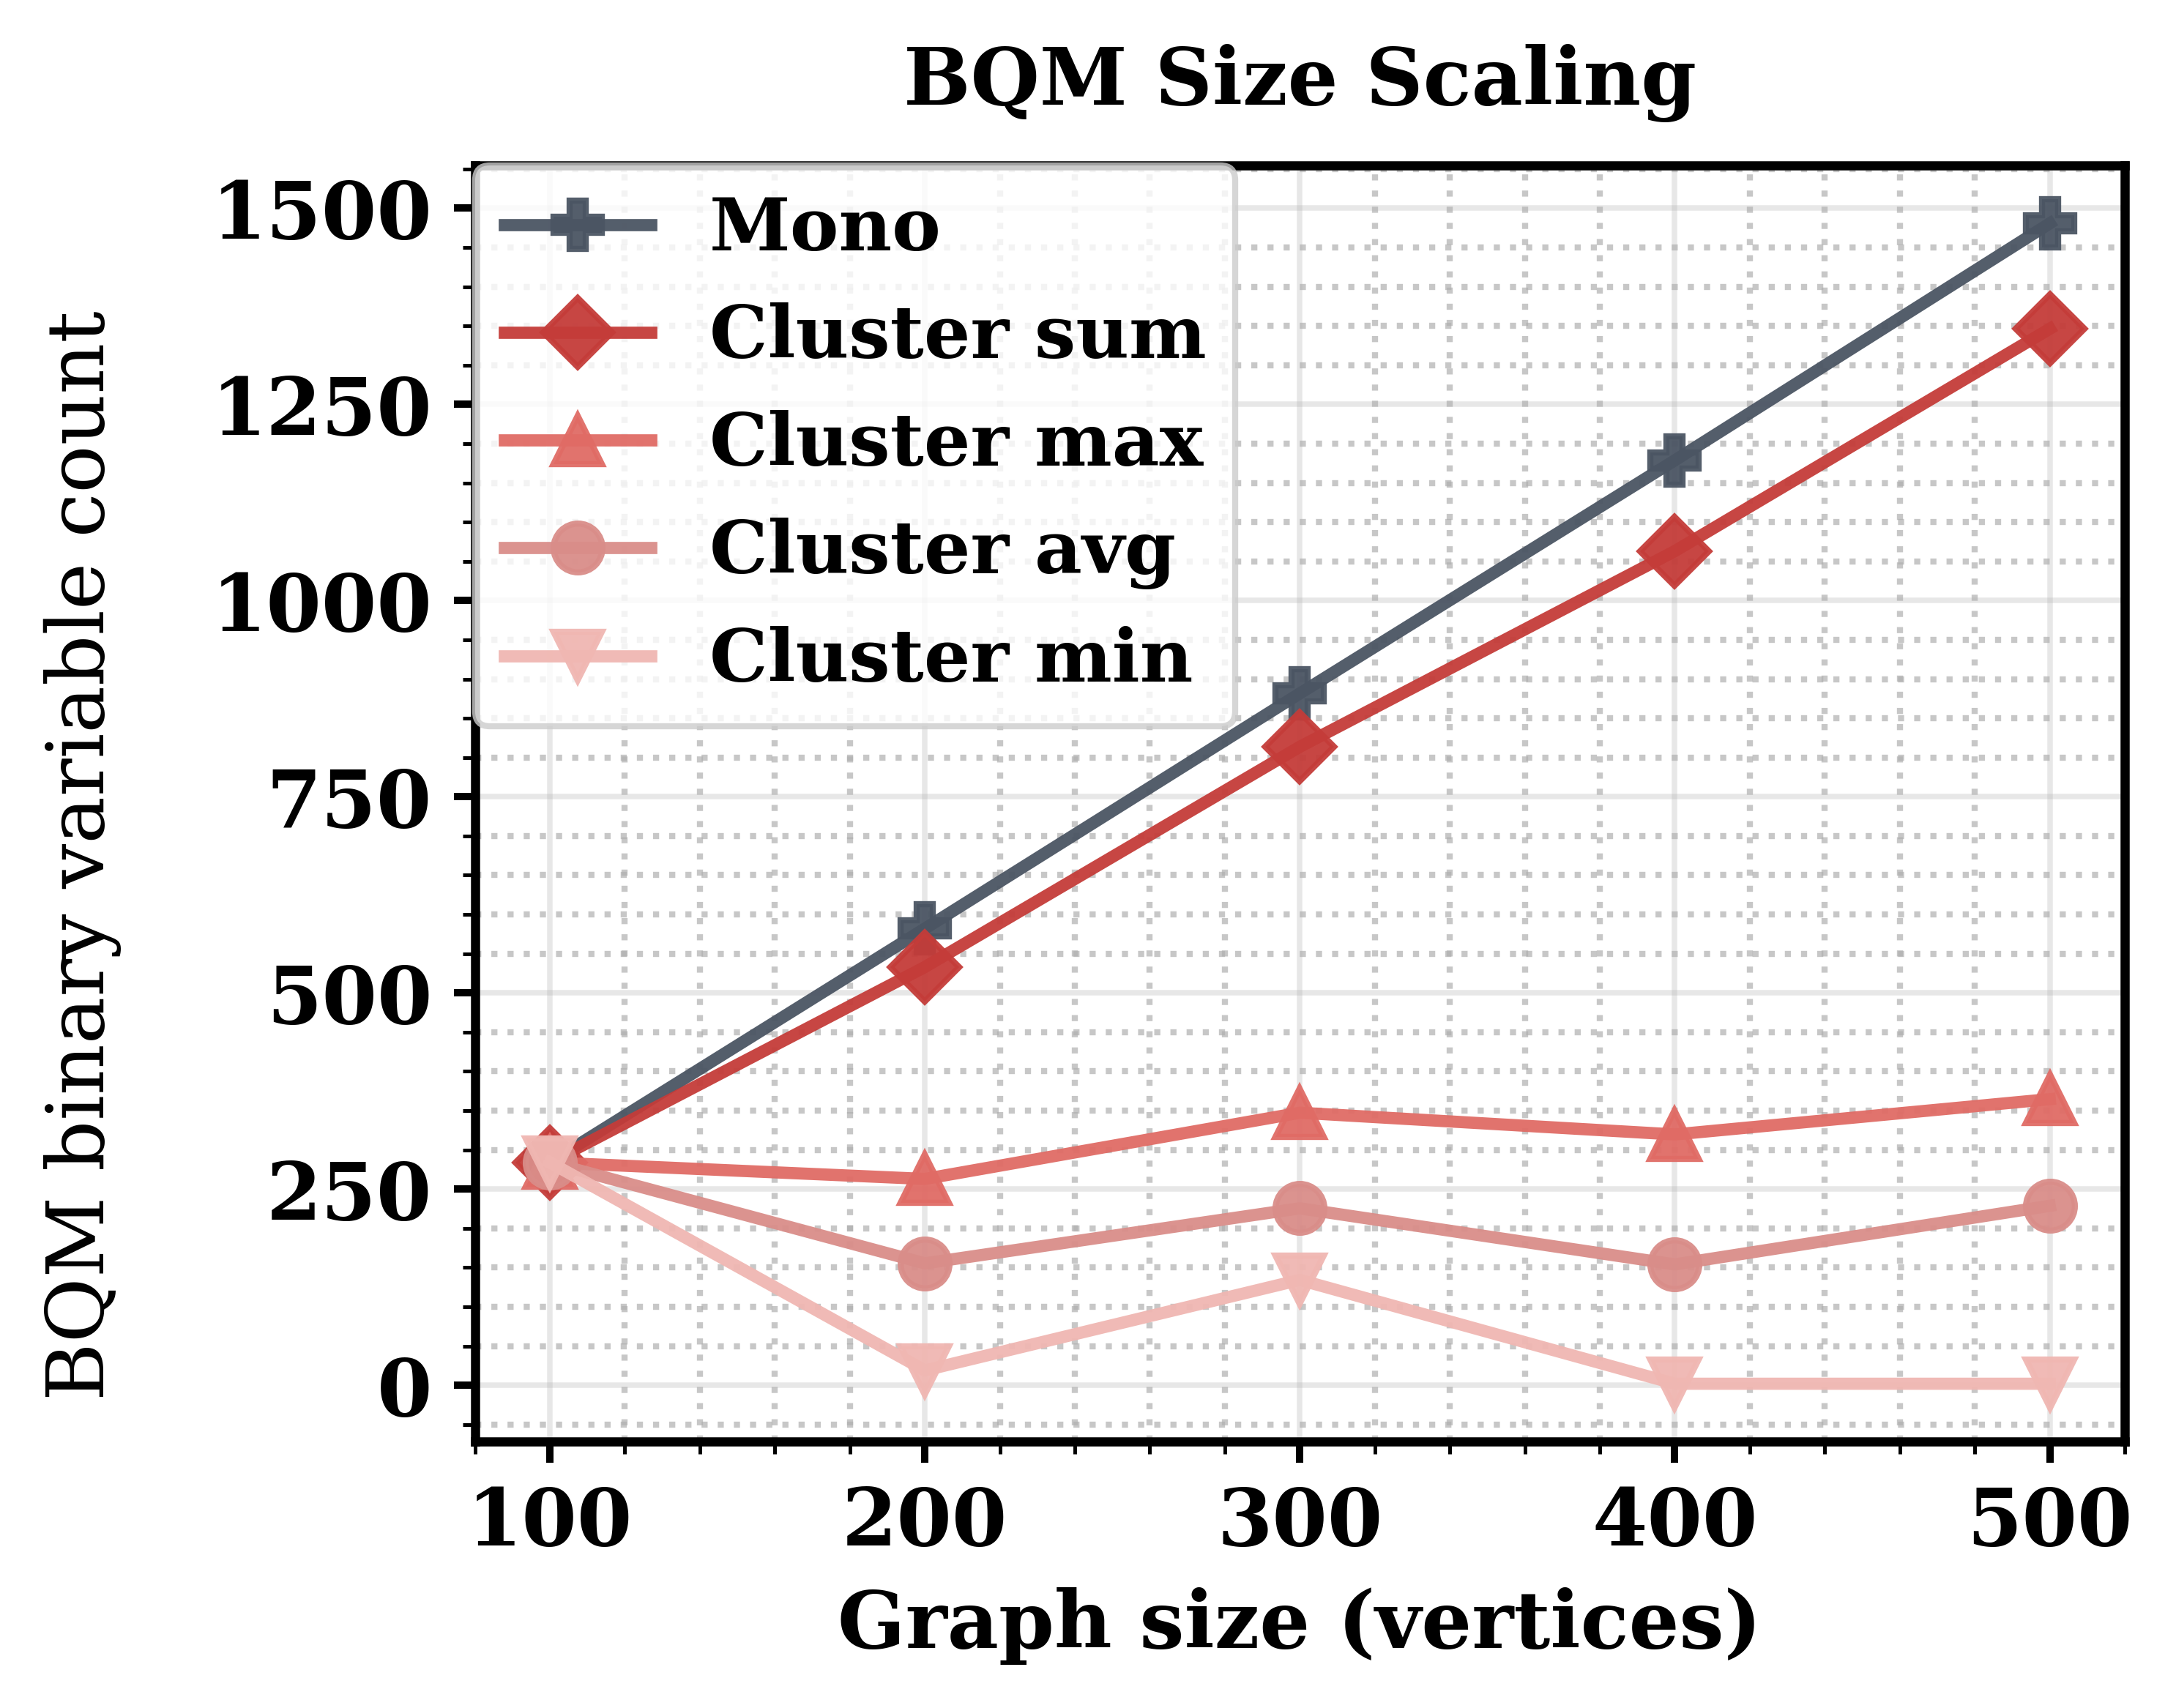
\includegraphics[width=\linewidth]{fig/scalability.png}
\caption{BQM 이진 변수 수. Mono는 분할하지 않은 경우이며, Cluster sum/max/avg/min은 분할 후 부분 그래프들의 합계와 최대·평균·최소이다.}
\label{fig:scalability}
\end{figure}

이 차이는 임베딩 가능 여부를 가른다. 분할하지 않은 경우 \(|V|=100\)에서는 평균 3{,}008개의 물리 큐비트로 임베딩되지만 \(|V|\geq200\)에서는 1{,}000초의 기본 탐색 예산 안에서 임베딩을 찾지 못한다(탐색 시간이 1{,}021--1{,}064초로 모두 예산에 붙어 있다). 이는 임베딩 불가능성의 증명이 아니라 휴리스틱 탐색의 실패이며, 예산을 늘리거나 다른 임베딩 알고리즘을 쓰면 결과가 달라질 수 있다. 반면 분할한 경우 \(|V|=500\)까지 모든 부분 그래프가 임베딩되며, 부분 그래프 하나가 쓰는 물리 큐비트는 최대 4{,}391개(\(|V|=300\), 논리 변수 405개)로 5{,}640개 안에 들어간다. 논리 변수 582개가 이상적 토폴로지에서 임베딩되지 않는 반면 428개가 더 열악한 실제 동작 그래프에서 4{,}181개의 물리 큐비트로 임베딩되는 것은 제~\ref{subsec:method_partition}절에서 예측한 커플러 우선 포화와 부합하는 방향이다. \(P_3\) 항이 거리 2의 간선 쌍까지 잇기 때문에 커플링 밀도가 변수 수보다 빠르게 늘어나기 때문이나, 이번 실험은 커플링 수를 기록하지 않아 직접 확인하지는 못했다.

\subsection{해 품질}

그림~\ref{fig:apsp}와 그림~\ref{fig:flow}는 \(D_{\mathrm{avg}}\)와 \(F_{\mathrm{bal}}\)을 방법별로 보여 준다. 강연결 배향은 Cluster, Global, ILS, Robbins가 15회 시행 전부에서, Raw SA는 \(|V|\leq300\)의 9회에서만 얻었다. Robbins는 강연결을 보장하지만 거리와 흐름 균형 모두에서 가장 나쁘다. Random은 무작위 표본(크기마다 30개, 총 150개) 가운데 강연결인 것이 하나도 없어 \(D_{\mathrm{avg}}\)를 정의할 수 없었으나, \(F_{\mathrm{bal}}\)은 575, 1{,}170, 1{,}765, 2{,}359, 2{,}943으로 오히려 Robbins보다 낫다(표에는 싣지 않았다). 강연결을 깊이 우선 탐색으로 강제하는 대가가 흐름 균형에서 두 배가량 든다는 뜻이다. Raw SA는 \(|V|\leq300\)에서 \(D_{\mathrm{avg}}\)가 낮지만 \(|V|\geq400\)에서는 강연결 배향을 얻지 못한다. 다만 이 우위는 계산량을 함께 보아야 한다. 우위가 성립하는 \(|V|\leq300\) 구간에서 Raw SA의 인스턴스당 탐색 시간은 Cluster 총 시간(분할·임베딩 탐색 + QUBO 풀이)의 4.7--11.8배이며, \(|V|=300\)에서 24{,}936초 대 2{,}584초다. Raw SA가 강연결 배향을 얻지 못하는 \(|V|=500\)에서는 101{,}597초 대 4{,}260초로 약 24배까지 벌어진다. \emph{ILS}는 모든 크기에서 \(D_{\mathrm{avg}}\)가 가장 낮은데, 이는 ILS가 평가 지표를 직접 최소화하는 반면 QUBO 계열은 대리 목적 \(H\)를 최소화하기 때문이다. ILS의 인스턴스당 시간은 \(|V|=500\)에서 44{,}862초로 Cluster 총 시간의 10.5배다.

\begin{figure}[t]
\centering
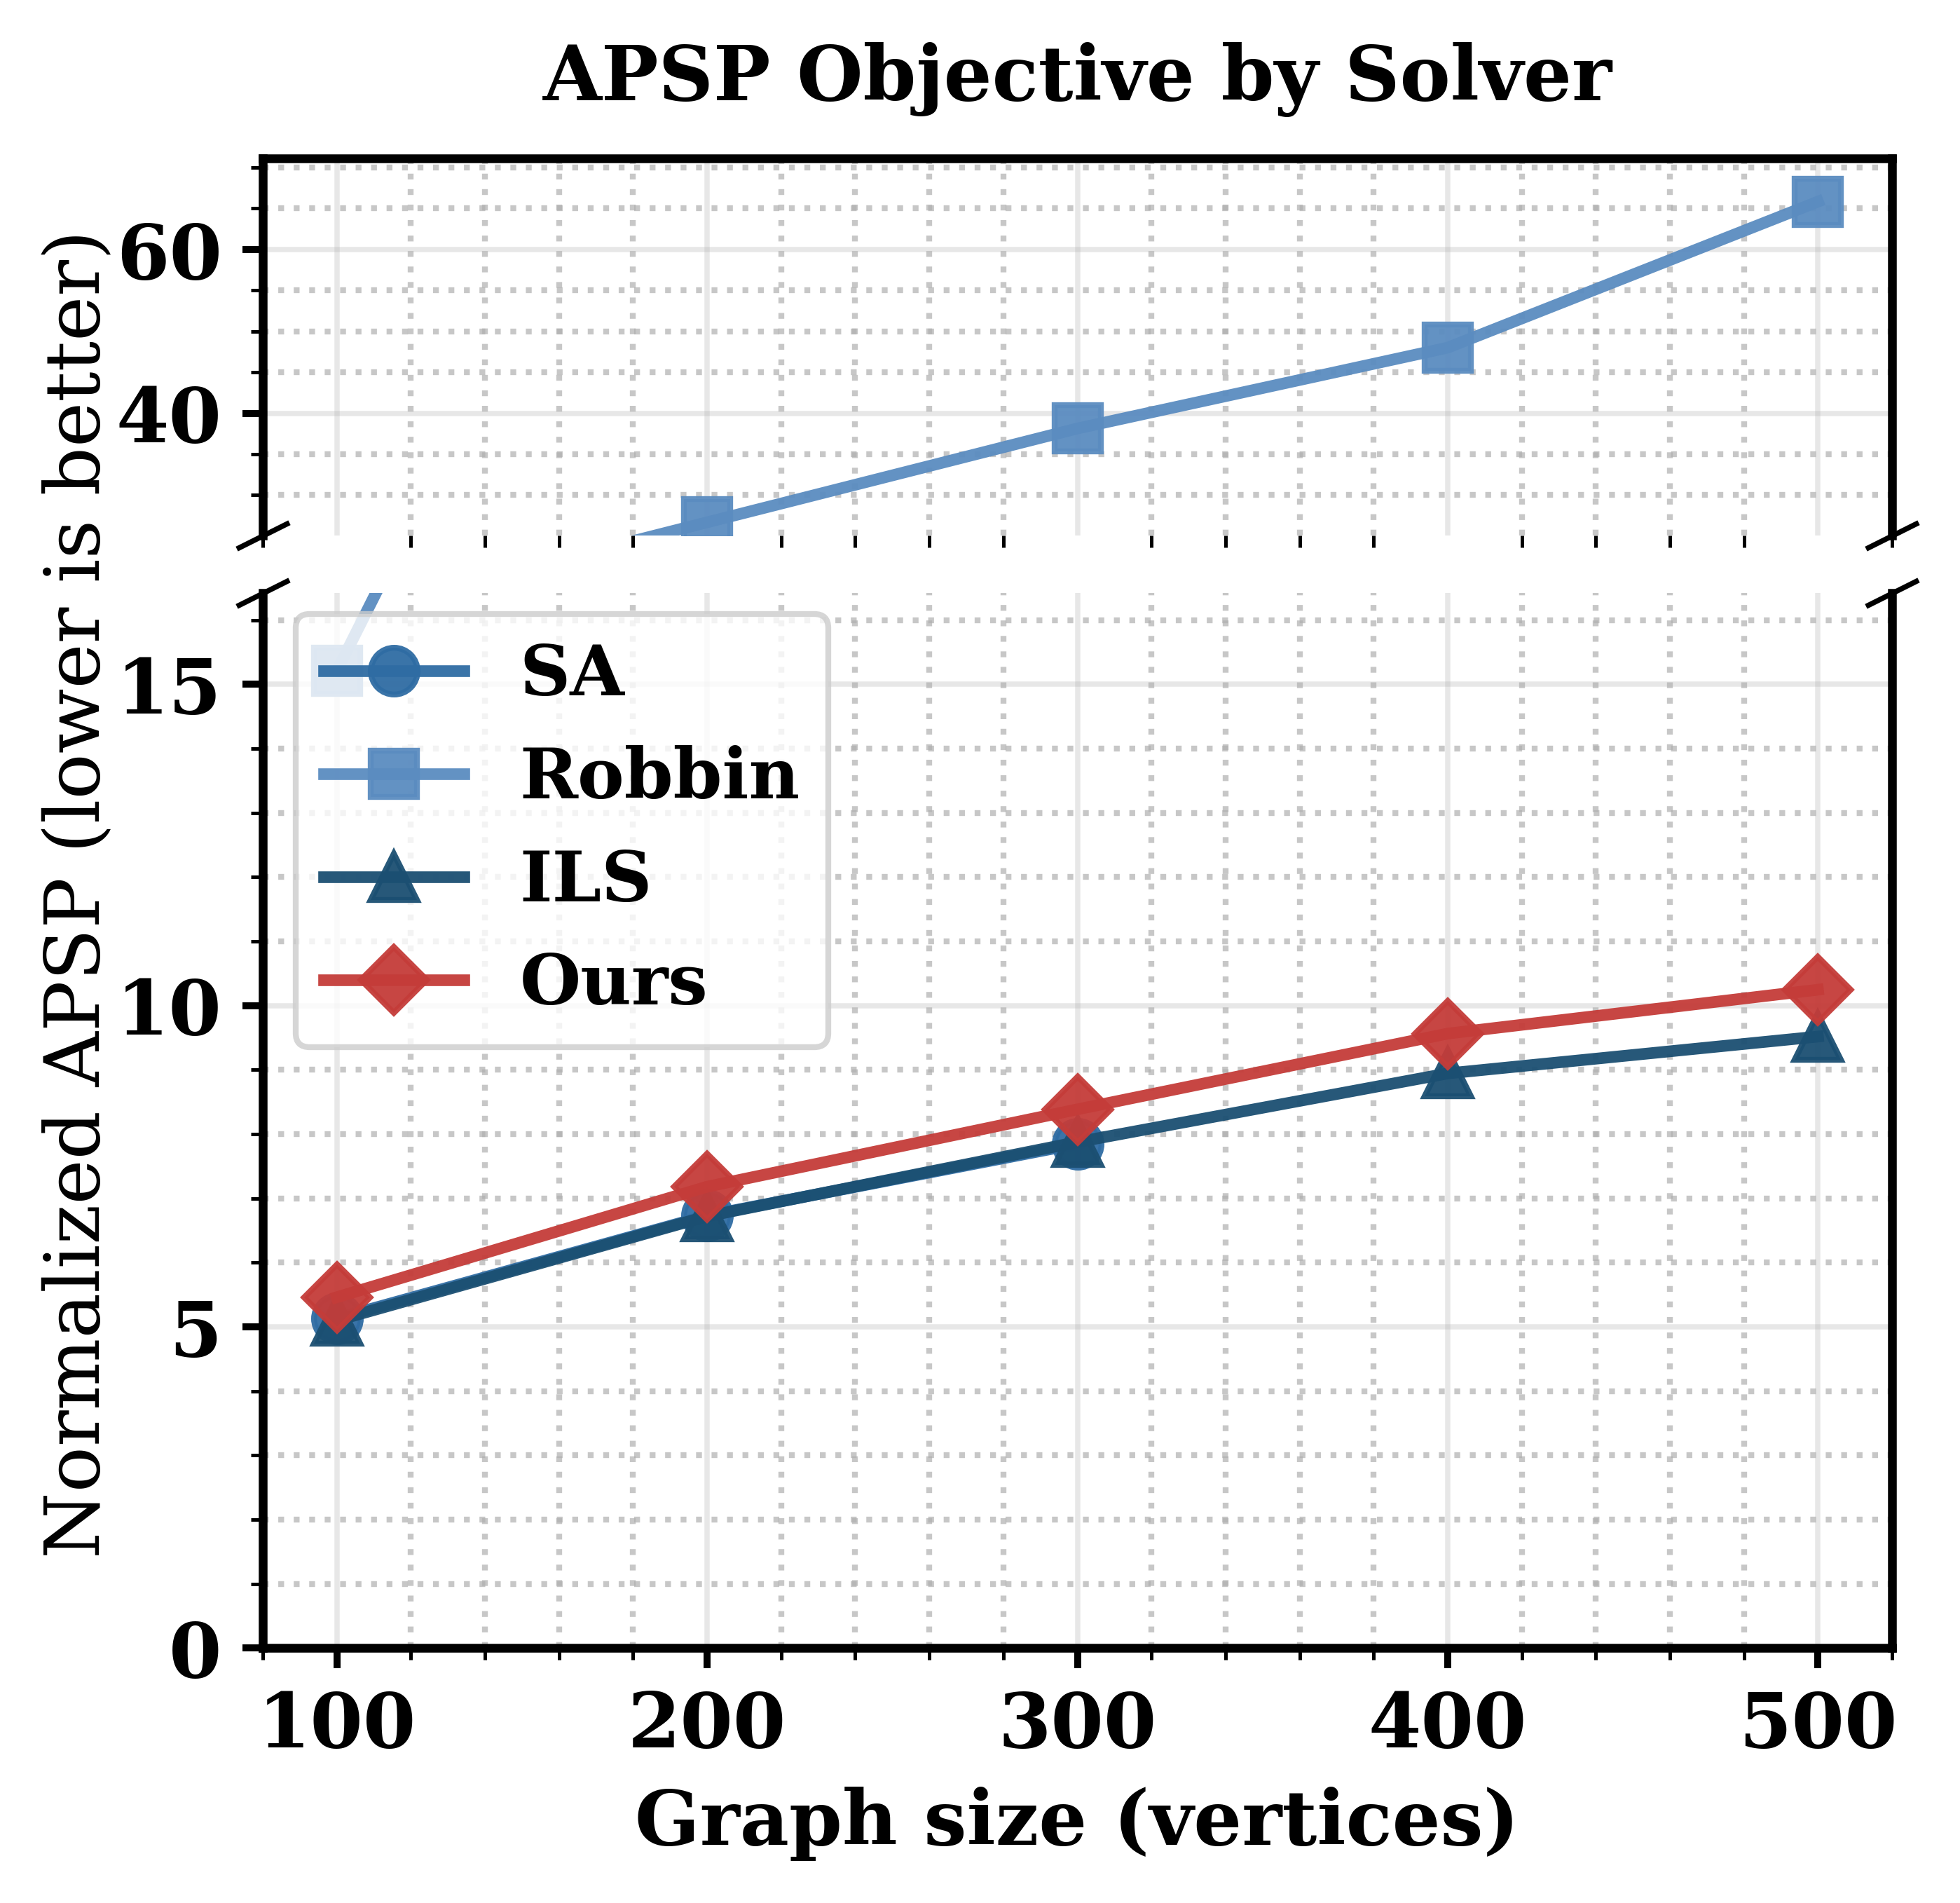
\includegraphics[width=\linewidth]{fig/apsp_reduction.png}
\caption{방향화 후 평균 유향 최단 경로 거리 \(D_{\mathrm{avg}}\)(낮을수록 좋음, 세 인스턴스 평균). SA는 Raw SA, Ours는 Cluster이다. Raw SA는 \(|V|\geq400\)에서 강연결 배향을 얻지 못해 표시하지 않았다.}
\label{fig:apsp}
\end{figure}

\begin{figure}[t]
\centering
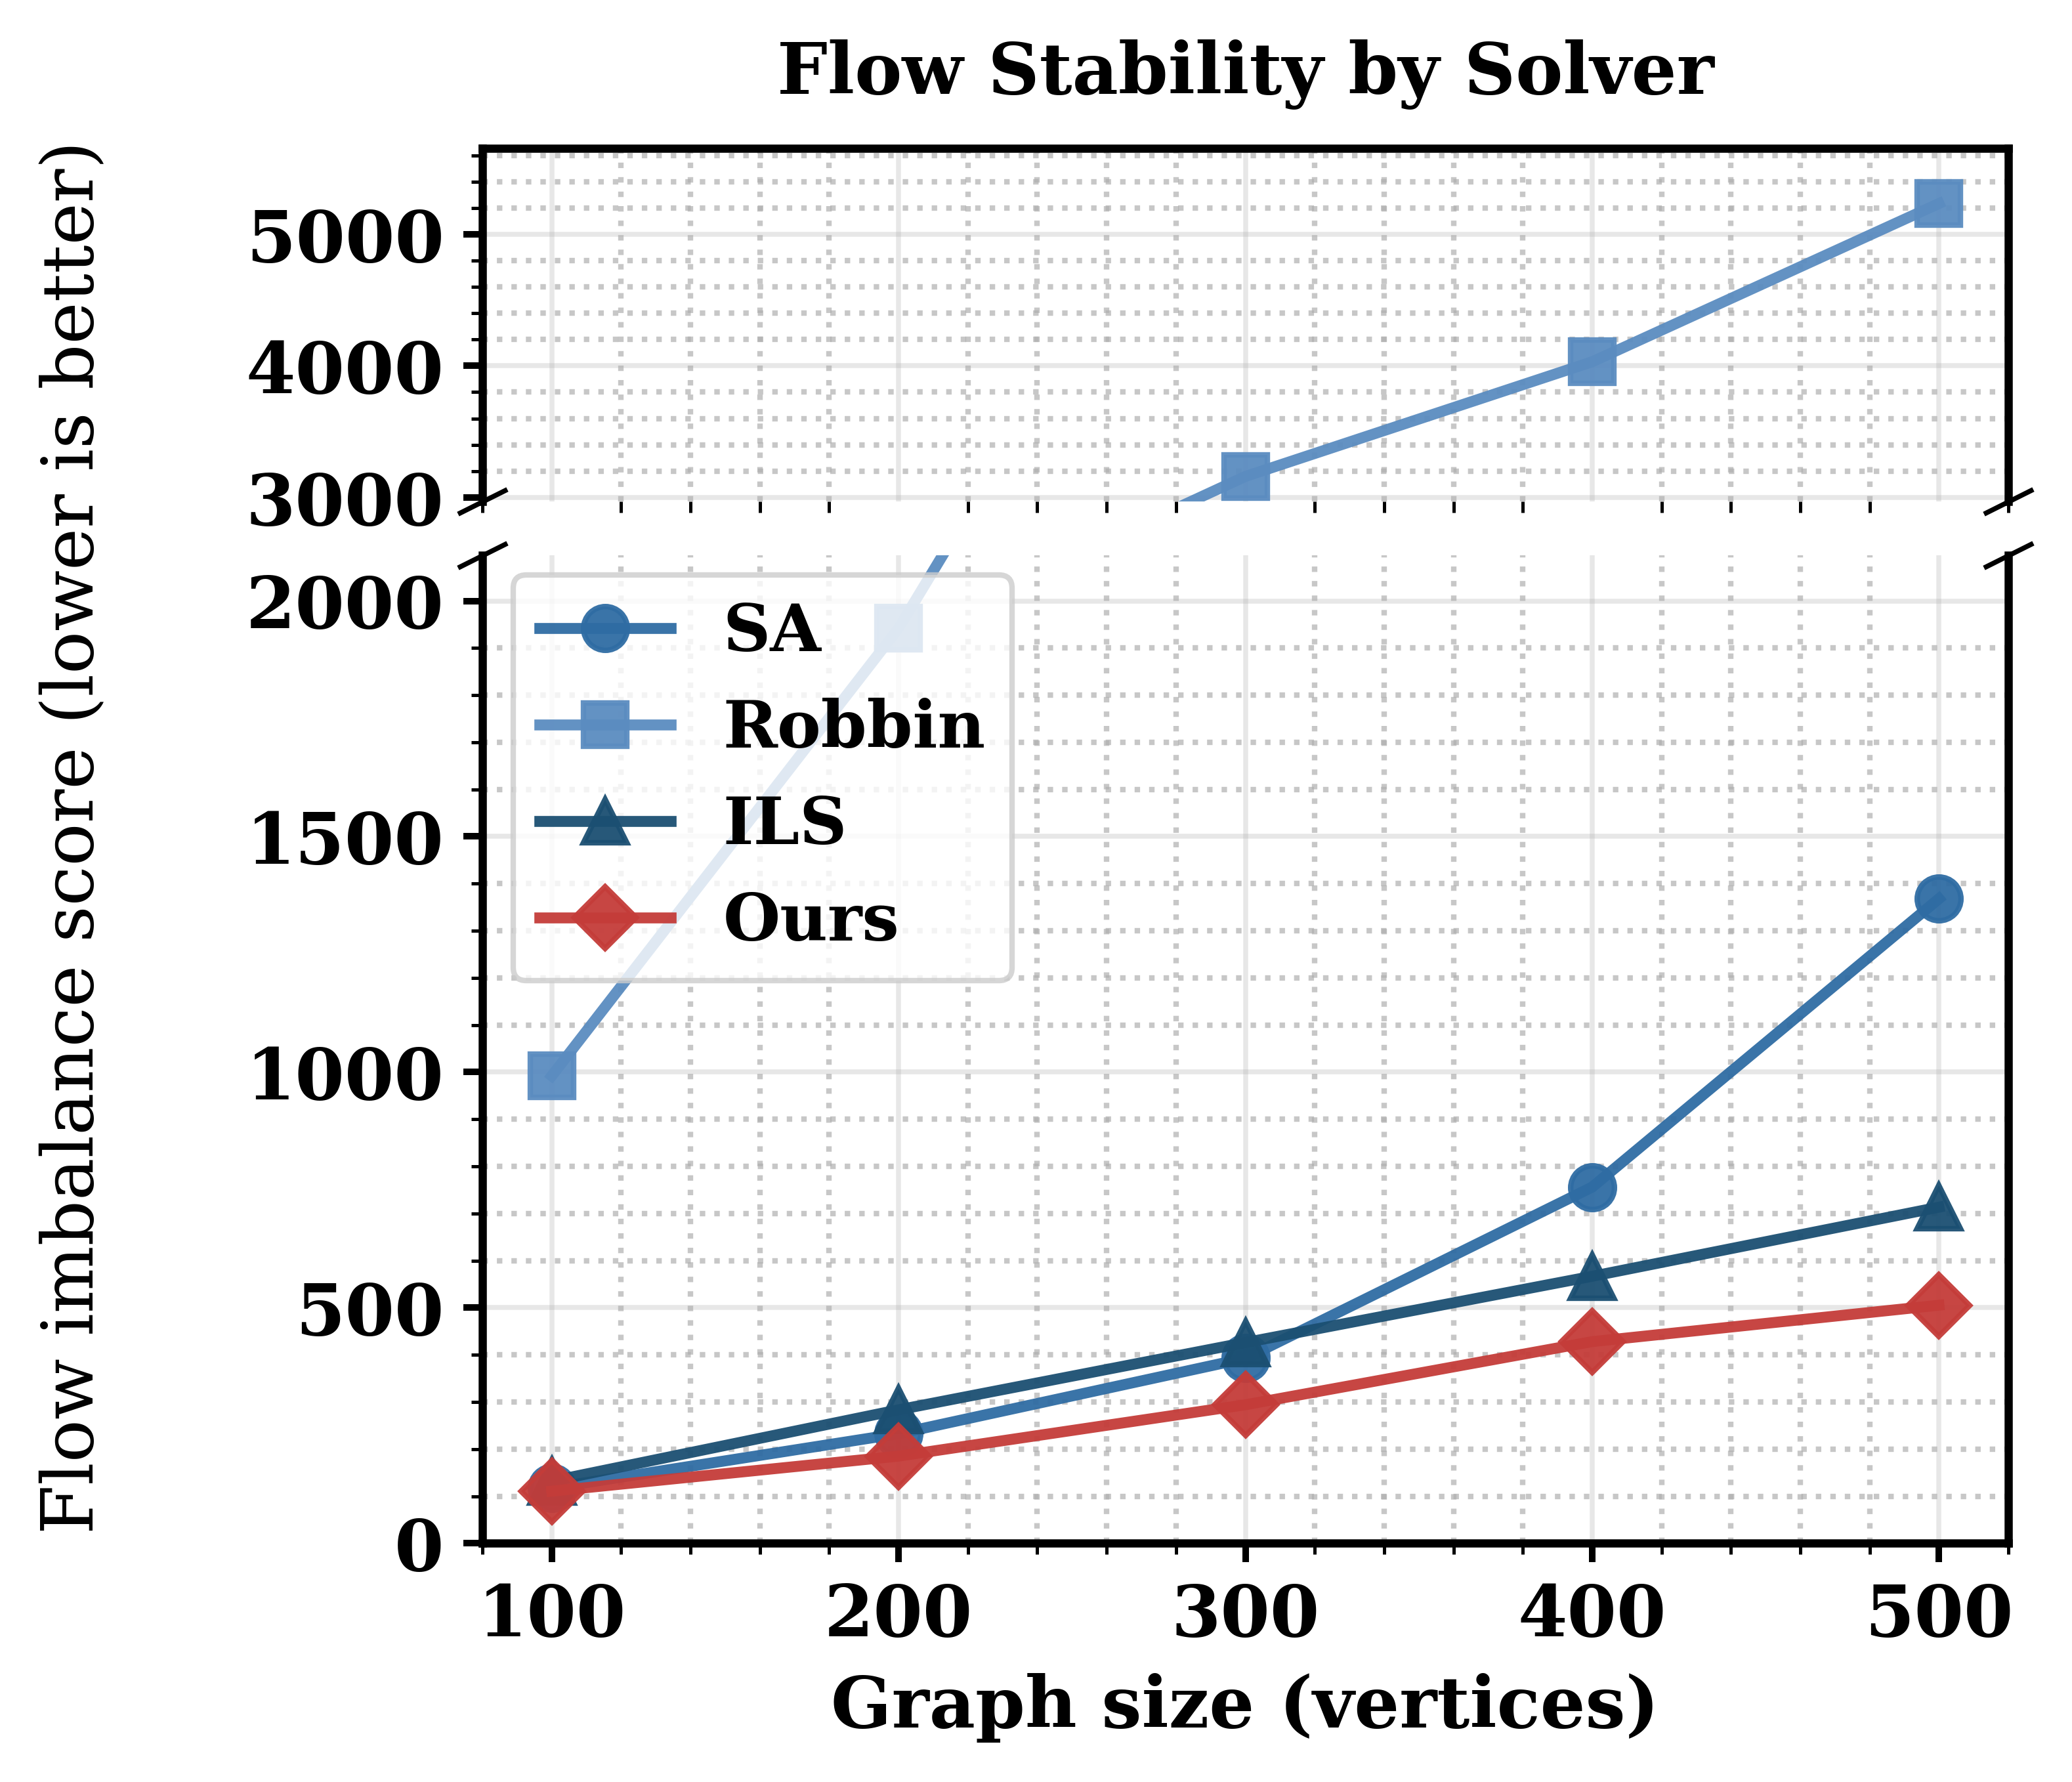
\includegraphics[width=\linewidth]{fig/flow_stability.png}
\caption{흐름 불균형 \(F_{\mathrm{bal}}\)(낮을수록 좋음, 세 인스턴스 평균).}
\label{fig:flow}
\end{figure}

QUBO 기반 두 방법을 비교하면 상반된 두 경향이 나타난다. 다만 \(|V|\geq200\)의 Global 값은 제~\ref{subsec:result_embed}절에서 임베딩되지 않은 QUBO를 고전 샘플러로 푼 결과이므로 현재 하드웨어에서 재현 가능한 수치가 아니다. \(D_{\mathrm{avg}}\)는 모든 크기에서 분할한 쪽이 근소하게 낮으나(\(|V|=500\)에서 10.25 대 10.46) 이 차이는 인스턴스 간 산포 안에 있다. \(|V|=500\)의 인스턴스별 값은 Cluster가 10.11/10.15/10.48, Global이 10.18/10.52/10.67로 두 분포가 겹치고 인스턴스가 셋뿐이므로 어느 쪽이 낫다고 주장하지 않는다. 반대로 \(F_{\mathrm{bal}}\)은 분할한 쪽이 두 배가량 나쁘다(505 대 245). 다만 이를 분해의 근사성으로 돌릴 수는 없다. \(|V|=100\)에서는 분할 탐색이 그래프 전체를 부분 그래프 하나로 반환하여 경계 간선이 하나도 없는데도 차이가 111 대 48로 오히려 가장 크고, 비율은 모든 크기에서 1.9--2.3배로 거의 일정하다. 경계 정점 누락이 원인이라면 \(|V|=100\)에서 차이가 사라지고 경계 비중과 함께 커져야 하므로 이 설명은 데이터와 맞지 않는다. 식~\eqref{eq:balhop}에서 \(F_{\mathrm{bal}}=\sum_vS_v^2-4P_2\)이고 \(\alpha=\beta=\lambda_2=\lambda_3=1\)에서 QUBO 에너지는 \(H=\mathrm{const}-5P_2-P_3\)이므로, \(F_{\mathrm{bal}}\)은 에너지 전체가 아니라 그 2-홉 성분에 상수를 더한 값이다. 따라서 이 차이는 QPU 표본의 \(P_2\)가 고전 시뮬레이티드 어닐링 표본보다 낮다는 것을 직접 뜻하며, 총 에너지의 대소는 \(P_3\)를 기록하지 않아 판정할 수 없다. 실제로 단위 가중치에서 \(F_{\mathrm{bal}}\)의 하한은 홀수 차수 정점의 수인데(제~\ref{subsec:model_flow}절), Global의 48, 99, 149, 192, 245는 모두 \(0.49|V|\) 부근으로 이 하한과 같은 규모인 반면 Cluster는 약 \(1.0|V|\)로 두 배 위에 있다. 특히 \(|V|=100\)에서는 분할이 일어나지 않아 두 arm이 동일한 284변수 BQM을 풀었으므로 이 크기의 비교는 분할 요인이 배제된 순수한 QPU 대 고전 SA 비교다. 그 조건에서 QPU는 \(D_{\mathrm{avg}}\)는 구분되지 않지만 \(F_{\mathrm{bal}}\)은 2.3배 나빴다. 즉 이 항에서는 QPU가 다항 시간에 도달 가능한 최적값을 재현하지 못했다.

\subsection{실행 시간}

인스턴스당 평균 실행 시간은 두 부분으로 나뉜다. QUBO 풀이 시간은 분할한 쪽이 \(|V|=500\)에서 16.9초로 분할하지 않은 429초보다 25배 빠르다. 반면 임베딩 탐색 시간은 분할한 쪽이 4{,}243초로 더 크다. 부분 그래프마다 탐색을 수행하기 때문이며, 분할하지 않은 경우의 1{,}064초는 대부분 실패로 끝나는 단일 탐색 비용이다. 고전 방법인 Robbins는 3.5초로 가장 빠르지만 그림~\ref{fig:apsp}에서 보듯 해 품질이 크게 떨어진다.

즉 현재 구현에서 지배적인 비용은 QUBO 풀이가 아니라 임베딩 탐색이다.

\subsection{\(n\)-홉 대리 목적의 타당성}

제~\ref{subsec:model_hop}절의 대리 목적이 실제로 거리와 연관되는지를 별도 실험으로 확인하였다. 실험과 같은 규모인 정점 100개, 간선 286개의 Delaunay 그래프에서 강연결 방향 조합 146개를 무작위로 뽑고, 각 조합의 유향 최단 경로 거리 합과 \(n\)-홉 도달 쌍 수를 함께 측정하였다. 여기서 \(n\)-홉 도달 쌍 수란 정확히 \(n\)개의 간선으로 이루어진 단순 경로가 존재하는 순서쌍의 수로, 가중 보행 수인 \(P_n\) 자체는 아니지만 단위 가중치에서 같은 구조를 세는 대리량이다.

\begin{figure}[t]
\centering
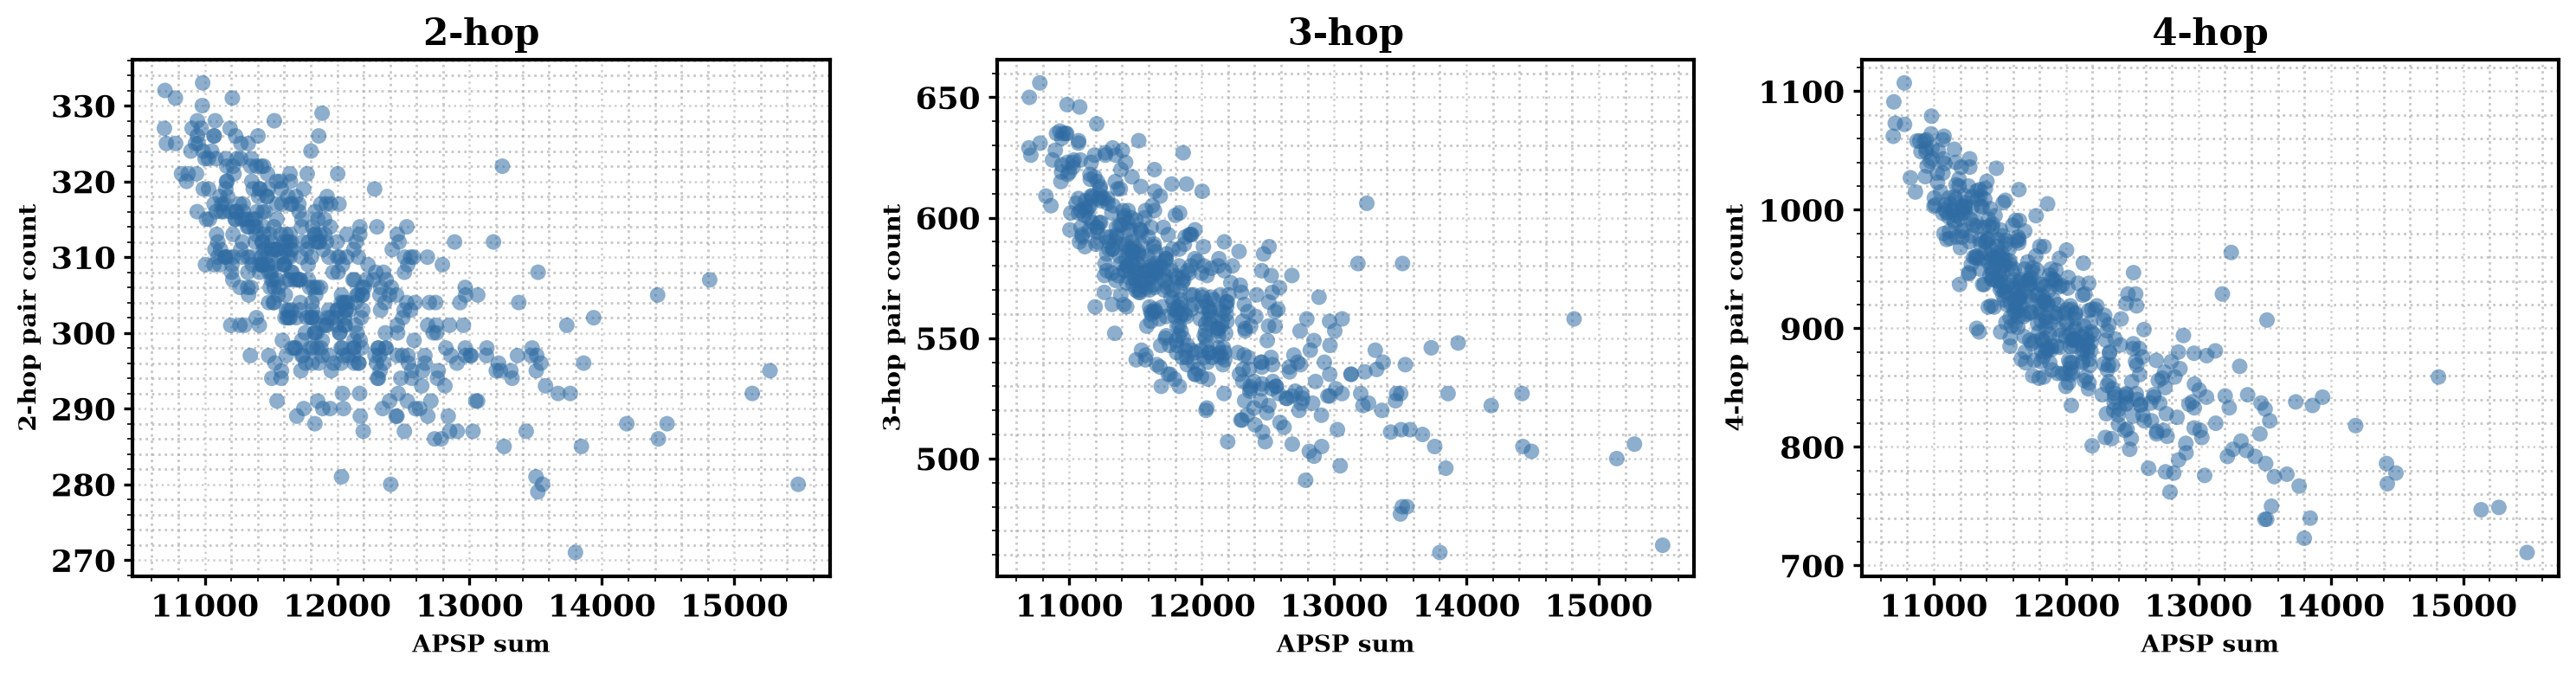
\includegraphics[width=\linewidth]{fig/nhop_apsp.png}
\caption{유향 최단 경로 거리 합과 \(n\)-홉 도달 쌍 수의 관계(정점 100개, 간선 286개, 방향 조합 146개). 왼쪽부터 \(n=2,3,4\).}
\label{fig:nhop}
\end{figure}

그림~\ref{fig:nhop}에서 세 홉 길이 모두 뚜렷한 음의 상관을 보인다. 즉 \(n\)-홉 도달 쌍이 많은 배향일수록 거리 합이 작으며, \(P_n\)의 최대화를 거리 최소화의 대리로 쓰는 것이 이 인스턴스에서 타당함을 뒷받침한다. 다만 상관의 세기만 놓고 보면 \(n=4\)가 \(n=2\)보다 낫다. 따라서 홉 길이를 \(\{2,3\}\)으로 한정한 근거는 상관의 우열이 아니라 명제~\ref{prop:deg}의 차수 조건이다. \(n=4\)를 넣으면 목적함수가 4차가 되어 차수 축소와 보조 변수가 필요해지고, 제~\ref{subsec:result_embed}절에서 이미 한계에 닿은 커플링 밀도가 더 늘어난다. 정점 50개 그래프에서도 같은 경향을 확인하였다. 단일 그래프 실험이므로 상관계수를 보고하지는 않는다.

\subsection{홉 길이 절제와 커플링 실측}

\(P_3\) 항의 비용과 이득을 분리하기 위해, 같은 15개 인스턴스에서 \(\lambda_3=1\)(hop23)과 \(\lambda_3=0\)(hop2)의 두 구성을 고전 시뮬레이티드 어닐링(표본 20개)으로 비교하였다. 그림~\ref{fig:ablation}이 결과를 요약한다.

\begin{figure}[t]
\centering
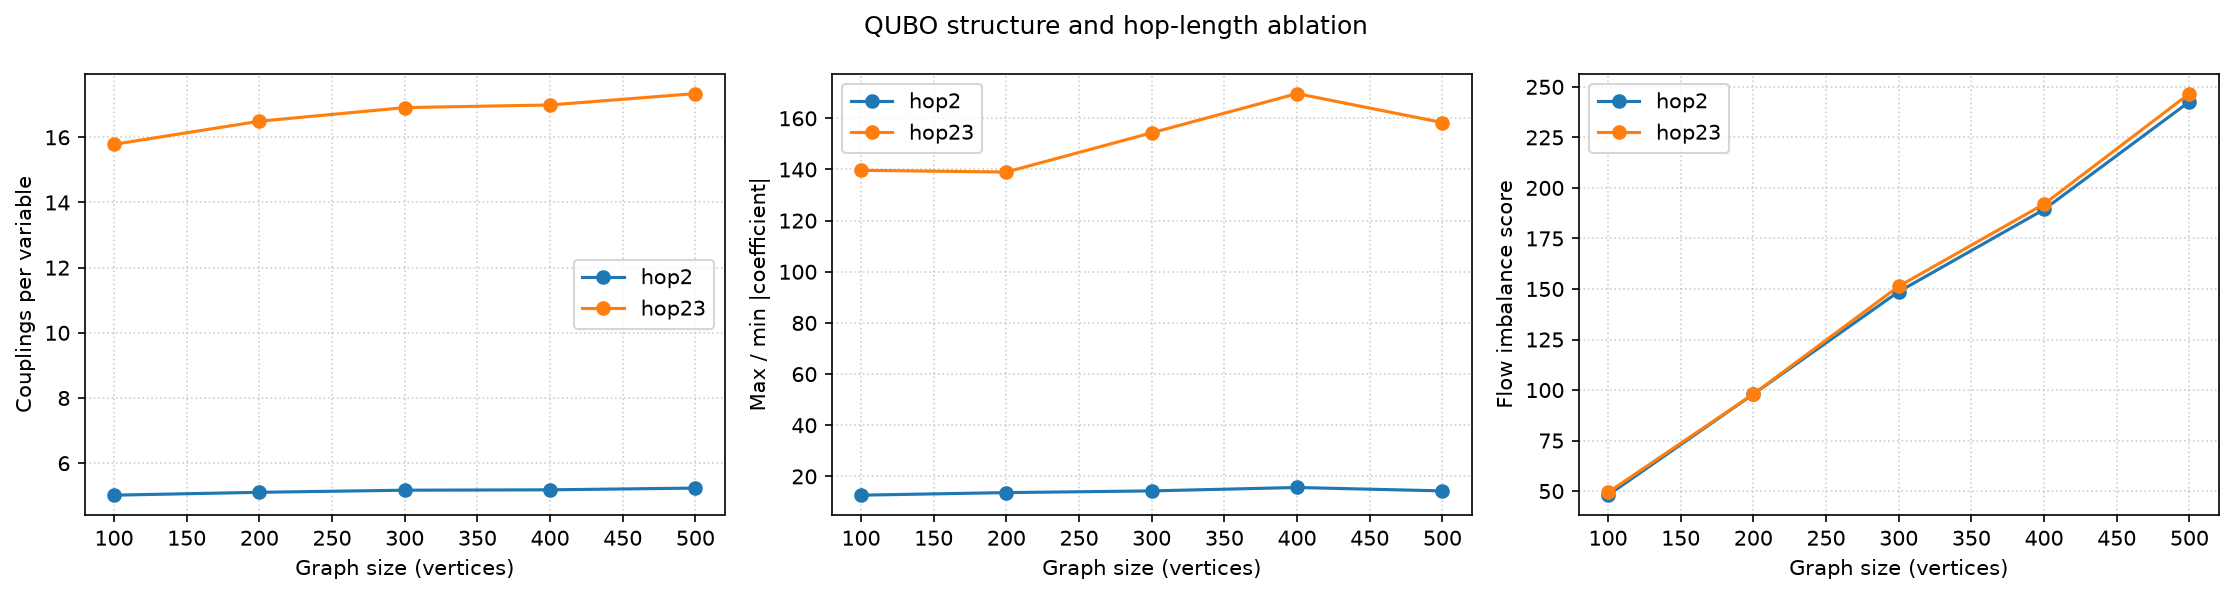
\includegraphics[width=\linewidth]{fig/qubo_structure.png}
\caption{홉 길이 절제. 왼쪽부터 변수당 커플링 수, 계수 최대·최소 비, 흐름 불균형. hop23은 \(\lambda_2=\lambda_3=1\), hop2는 \(\lambda_3=0\)이다.}
\label{fig:ablation}
\end{figure}

비용 쪽은 뚜렷하다. \(P_3\)를 포함하면 변수당 커플링 수가 5.0--5.2에서 15.8--17.3으로 3.2배가 되고, 계수 최대·최소 비가 13--16에서 140--170으로 한 자릿수 커지며, 풀이 시간도 \(|V|=500\)에서 97초 대 311초로 3.2배다. 제~\ref{subsec:method_partition}절이 예고한 커플링 실측이 이것으로, \(|V|=500\)에서 커플링 수는 간선 수의 약 17배인 25{,}678개다.

이득 쪽은 관측되지 않았다. 15개 인스턴스에서 거리 합은 hop23이 8회, hop2가 7회 낮았고 최대 차이가 1.1\%로 인스턴스 산포 안이다. 흐름 불균형은 hop23이 나은 경우가 한 번도 없었으며(7회 열세, 8회 동률), 강연결은 양쪽 모두 15회 전부 달성했다. 즉 이 인스턴스군에서 \(P_3\)는 제~\ref{subsec:result_embed}절의 임베딩 한계를 만드는 커플링 밀도를 3배로 키우면서 해 품질을 개선하지 못했다. \(\lambda_3=0\) 구성이 분할 없이도 더 큰 그래프를 임베딩할 수 있는지는 후속 과제로 남긴다.

\subsection{보고하지 못한 항목}

Cluster의 \(|V|=200\) 시행 셋 중 하나는 분할 단계에서 중단되어 해당 크기의 품질 지표만 두 인스턴스 평균이다(실행 시간과 큐비트 수는 셋 모두 포함). 대상이 Delaunay 삼각분할이라 차수 2 정점이 거의 없어 직렬 축약은 작동하지 않았으며, 따라서 제~\ref{subsec:method_pre}절의 축약 관련 요소와 평행 간선 사례는 이번 실험의 검증 범위 밖이다.

\section{결론} \label{sec:conclusion}

\bibliographystyle{plain}
\bibliography{../../AQC/Fig_MaiDinhCong/ref}

\end{document}
